%%%%%%%%%%%%%%%%%%%%%%%%%%%%%%%%%%%%%%%%%
% Diaz Essay
% LaTeX Template
% Version 2.0 (13/1/19)
%
% This template originates from:
% http://www.LaTeXTemplates.com
%
% Authors:
% Vel (vel@LaTeXTemplates.com)
% Nicolas Diaz (nsdiaz@uc.cl)
%
% License:
% CC BY-NC-SA 3.0 (http://creativecommons.org/licenses/by-nc-sa/3.0/)
%
%%%%%%%%%%%%%%%%%%%%%%%%%%%%%%%%%%%%%%%%%

%----------------------------------------------------------------------------------------
%	PACKAGES AND OTHER DOCUMENT CONFIGURATIONS
%----------------------------------------------------------------------------------------
\documentclass[11pt]{diazessay} % Font size (can be 10pt, 11pt or 12pt)
\usepackage{graphicx}
\usepackage{array}
\usepackage{tabularx}
\usepackage{float}
\usepackage{csquotes}
\usepackage{csquotes}
\usepackage{listings}
\usepackage{xcolor}
\lstset { %
    language=C++,
    backgroundcolor=\color{black!5}, % set backgroundcolor%
    basicstyle=\footnotesize,% basic font setting
    breaklines=true,
}
%----------------------------------------------------------------------------------------
%	TITLE SECTION
%----------------------------------------------------------------------------------------

\title{\textbf{Trabajo Práctico} \\ {\Large\itshape Analisis de Circuitos}} % Title and subtitle

\author{\textbf{Cotarelo Rodrigo} \\ \textit{Facultad de Ingeniería, Universidad de Buenos Aires}} % Author and institution

\date{\today} % Date, use \date{} for no date



%----------------------------------------------------------------------------------------

\begin{document}

\vbox{
    \centering
    \maketitle %this typesets the contents of \title, \author and \date
    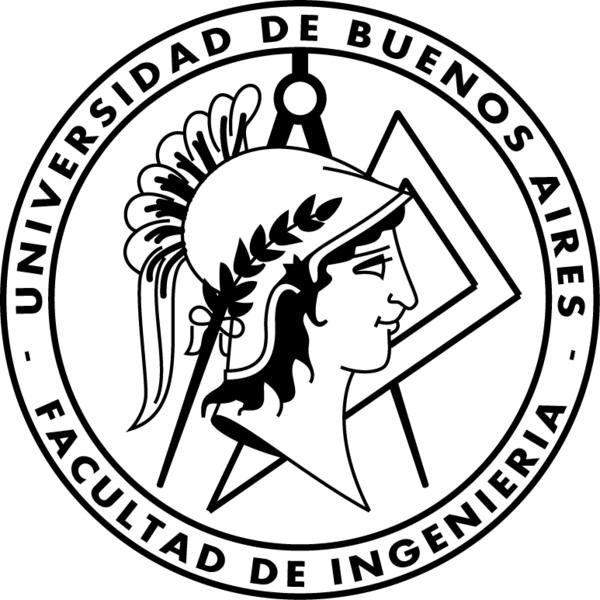
\includegraphics[width=0.5\textwidth]{Figures/fiuba.png}
}


%----------------------------------------------------------------------------------------
%	ESSAY BODY
%----------------------------------------------------------------------------------------
\newpage
\section*{Definir tipo de filtro}

\begin{equation}
H(s) = \frac{6,317 \cdot 10^8 \cdot s^2}{s^4 + 3,554 \cdot 10^4 \cdot s^3 + 1,895 \cdot 10^9 \cdot s^2 + 2,245 \cdot 10^{13} \cdot s + 3,99 \cdot 10^{17}} 
\end{equation}

En un primer analisis podemos indentificar que se trata de un filtro pasa-banda ya que tendiendo a infinito o menos infinito podemos 
ver que la transferencia es cero. Ademas como tenemos un cero en cero sabemos que hay una subida de ganancia que luego tiene que ser atenuada y es por esto
que lo podemos diferenciar de un pasa-bajos por ejemplo.\\
\\
Esta compuesto por 4 polos los cuales son dos pares complejos conjugados:
\begin{itemize}
	\item -12002.32+34212.9j\\
	\item -12002.32-34212.9j\\
	\item -5767.68+16439.38j\\
	\item -5767.68-16439.38j
\end{itemize}

Como los polos complejos conjugadores se consideran como un polo real doble y sabiendo como se conforma el diagrama asintotico sabemos que existen
dos caidas en la transferencia (una por cada polo doble) con pendiente -40db y una subida de 40db gracias al cero doble. Esto se corresponde con el
grafico de pasabanda que esperamos obtener.

La transferencia puede expresarse como la multiplicacion de dos transferencia de orden dos como se muestra a continuacion:
\begin{equation}
H(s) = H_{0} \cdot \frac{ 2 \cdot \alpha_{1} \cdot s }{ s^2 + 2 \cdot \alpha_{1} \cdot s + w_{1}^2} \cdot \frac{ 2 \cdot \alpha_{2} \cdot s }{ s^2 + 2 \cdot \alpha_{2} \cdot s + w_{2}^2}
\end{equation}
\begin{itemize}
\item Expresion pasa-bajos 2 orden:
\begin{equation}
H = \frac{ 2 \cdot \alpha \cdot s }{ s^2 + 2 \cdot \alpha \cdot s + w^2}
\end{equation}
\begin{equation}
Q = \frac{w}{2 \cdot \alpha}
\end{equation}
\begin{equation}
f = \frac{w}{2 \cdot \pi}
\end{equation}\\
\item El primer pasabajos de orden 2:
\begin{equation}
H_{1} = \frac{24004.64 \cdot s^2}{s^2 + 24004.6 \cdot s + 1314578211.7924} 
\end{equation}
$\alpha_{1}$ = 12002.32\\
$w_{1}$ = 36257.11\\
$f_{1}$ = 5770.5\\
$Q_{1}$ = 1.51\\
\item El segundo pasabajos de orden 2:
\begin{equation}
H_{2} = \frac{11535.36 \cdot s^2}{s^2 +11535.36 \cdot s + 303519347.3668} 
\end{equation}
$\alpha_{2}$ = 5767.68\\
$w_{2}$ = 17421.81\\
$f_{2}$ = 2772.77\\
$Q_{2}$ = 1.51\\
\item Comparando las transferencias
\begin{equation}
6,317 \cdot 10^8 = H_{0} \cdot 2\alpha_{1} \cdot 2\alpha_{2}
\end{equation}
\begin{equation}
H_{0} = 2.28
\end{equation}
\end{itemize}

\newpage
\section*{Simulacion}
\begin{itemize}
\item Diagrama de Bode de modulo y fase \\
Podemos confirmar lo explicado anteriormente. El gráfico muestra claramente la subida de 40 db por década que después se compensa con el primer polo doble generando una meseta y en el segundo polo doble se produce la caída de -40 db por década.\\
\begin{figure}[h]
	\centering
	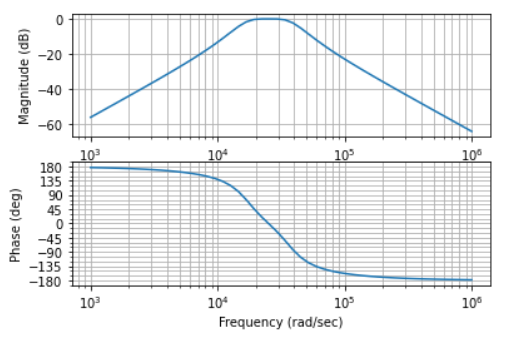
\includegraphics[width=\textwidth]{Bode.png}
\caption{Diagrama de Bode de modulo y fase}
\end{figure}\\
\newpage
\item Respuesta al escalon
\begin{figure}[h]
	\centering
	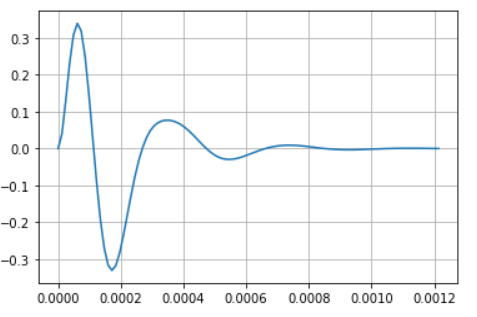
\includegraphics[width=\textwidth]{Respuesta_al_escalon.png}
\caption{Respuesta al escalon.}
\end{figure}
\newpage
\item Respuesta al impulso
\begin{figure}[h]
	\centering
	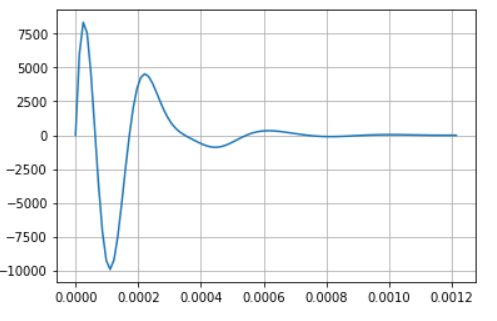
\includegraphics[width=\textwidth]{Respuesta_al_impulso.png}
\caption{Respuesta al impulso.}
\end{figure}
\item Respuesta a la senoidal \\
\\
Al tener un filtro pasabanda vamos a utilizar una frecuencia f0 = 4200Hz que esta dentro de nuestro ancho de banda y esperamos que el filtro atenue las senionadales con frecuencia de 1 decada mayor y menor.
\begin{figure}[h]
	\centering
	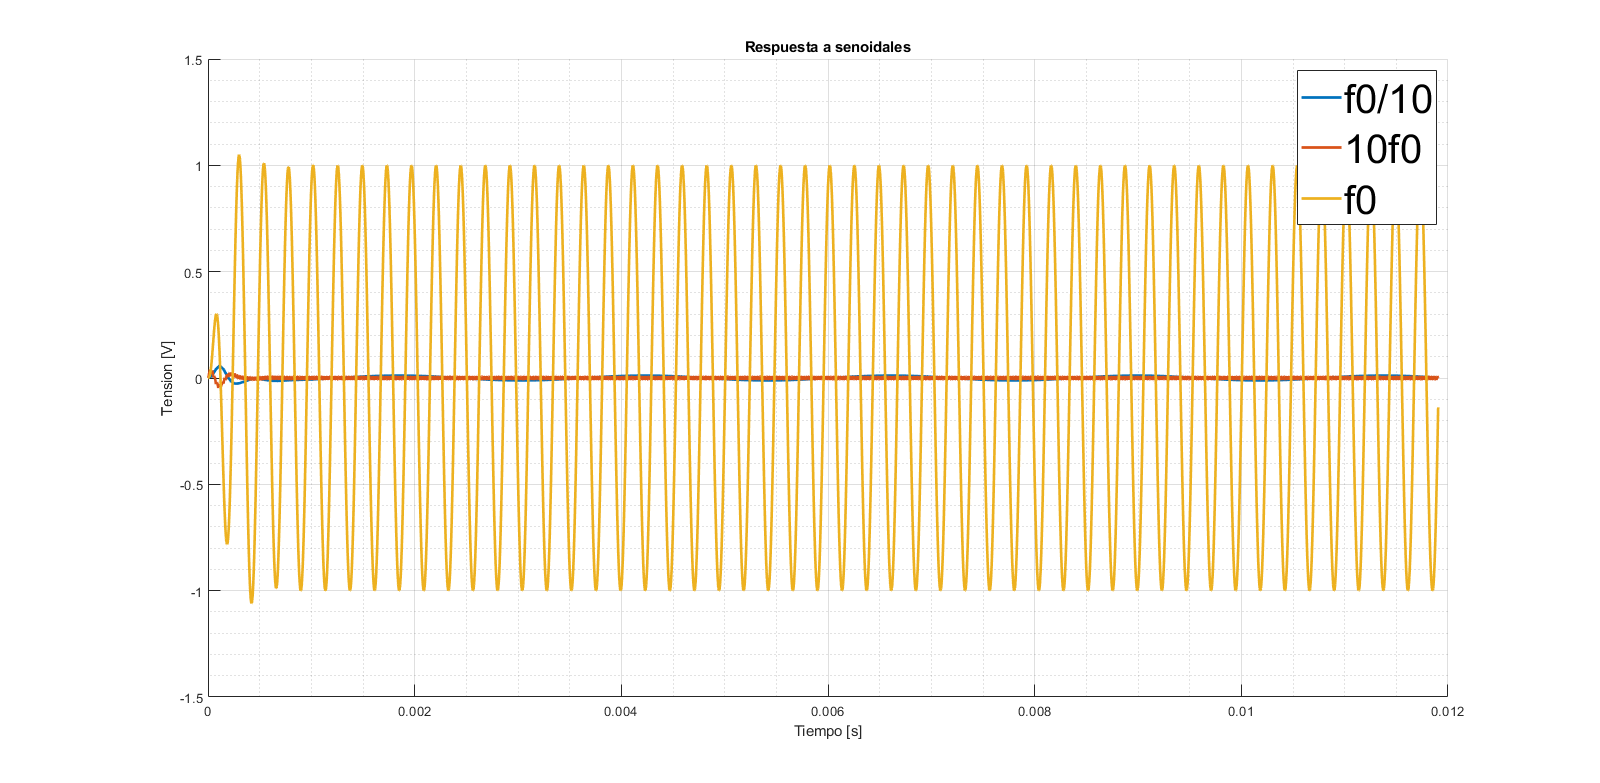
\includegraphics[width=\textwidth]{Respuesta_senoidal.png}
\caption{Respuesta a señal senoidal.}
\end{figure}
\newpage
\item Respuesta a la cuadrada
\begin{itemize}
\item f0 = 4200 \\
	\begin{figure}[h]
		\centering
			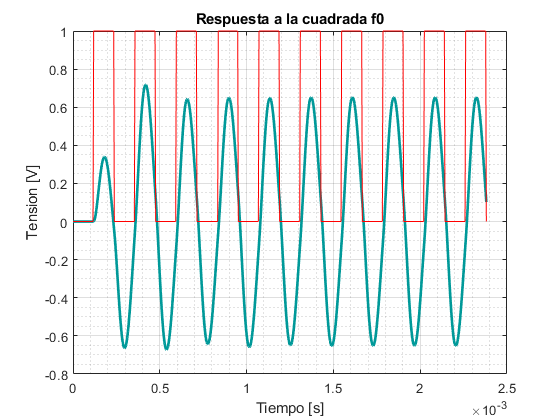
\includegraphics[width=\textwidth]{cuadrada_f0.png}
	\caption{Respuesta cuadrada.}
	\end{figure}

\item f0/10
	\begin{figure}[h]
		\centering
			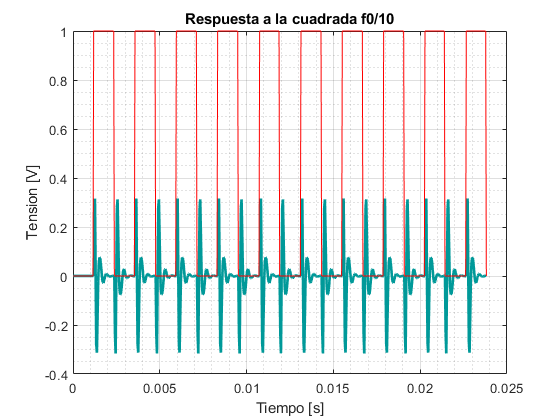
\includegraphics[width=\textwidth]{cuadrada_f0_div_10.png}
	\caption{Respuesta cuadrada.}
	\end{figure}
\newpage
\item 10 $\cdot$ f0 \\
	\begin{figure}[h]
		\centering
			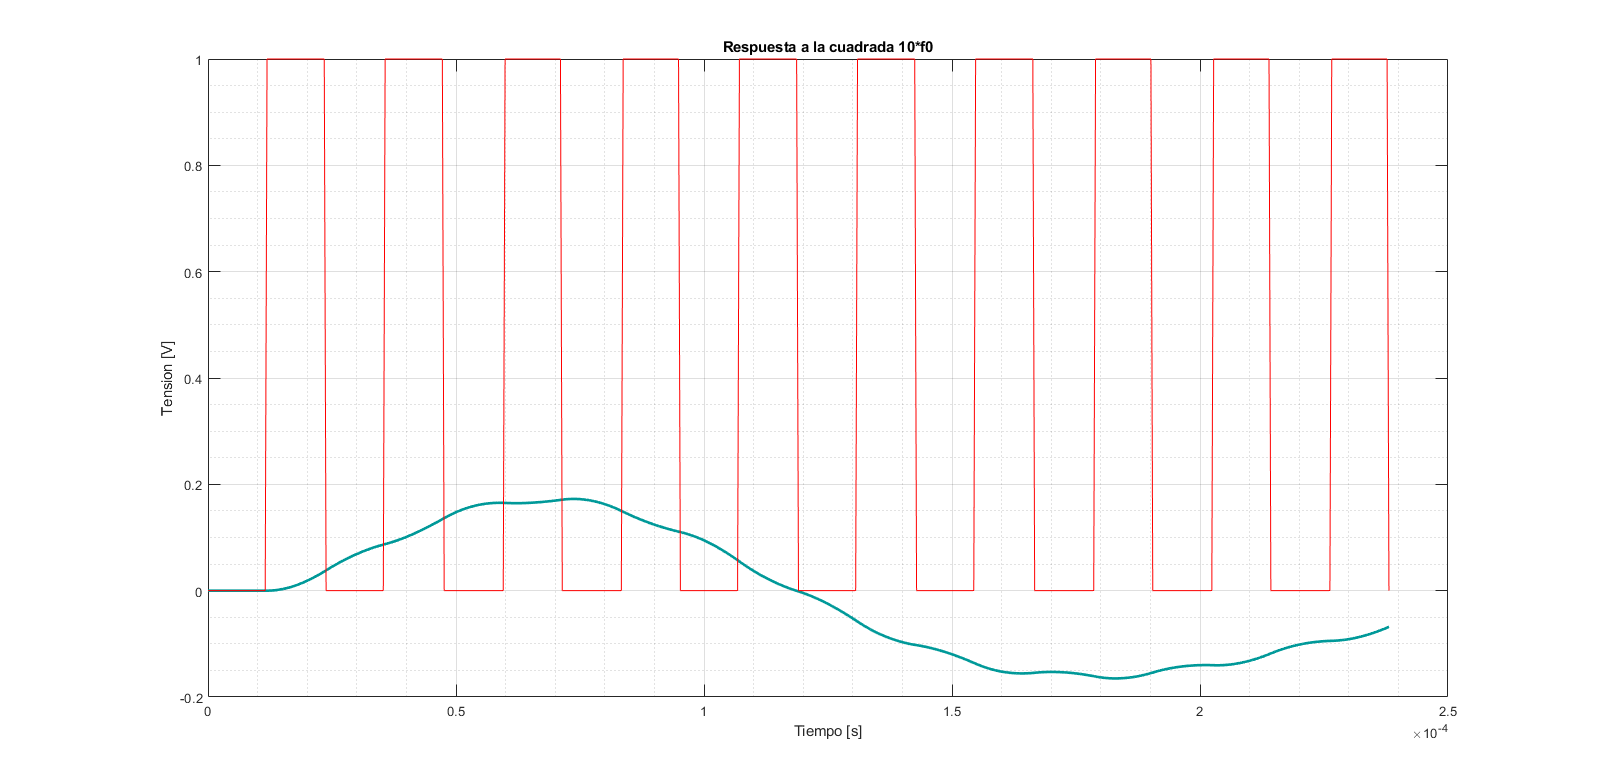
\includegraphics[width=\textwidth]{cuadrada_f0_por_10.png}
	\caption{Respuesta cuadrada.}
	\end{figure}
\end{itemize}
\end{itemize}

\newpage
\section*{Eleccion de circuito}
Para implementar este filtro se uso un pasabanda "Infinite Gain Multiple Feedback" ya que permite trabajar con cualquier factor de calidad Q.
\begin{figure}[h]
\centering
	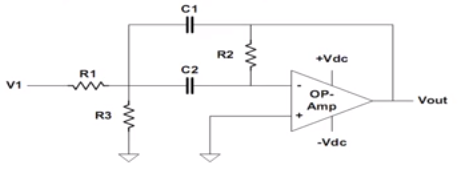
\includegraphics[width=\textwidth]{filtro.png}
\caption{Infinite Gain Multiple Feedback}
\end{figure}

\newpage
\section*{Valores normalizados}
En base a las ecuaciones del circuito presentadas arriba se calcularon los valores necesarios de los componentes junto a sus valores
normalizados respectivamente.\\
\break
\begin{tabular}{ |p{2cm}||p{2cm}|p{6cm}|  }
 \hline
 \multicolumn{3}{|c|}{Filtro pasabajos 1} \\
 \hline
 Componente&Valor&Valor Normalizado\\
 \hline
 C  & 12nF & 12nF\\
 R2  & 6.94k & 6.8k\\
 R1  & 2.30k & 2.2k\\
 R3  & 1.13k & 1.2k\\
 \hline
\end{tabular}\\
\break
\break
\begin{tabular}{ |p{2cm}||p{2cm}|p{6cm}|  }
 \hline
 \multicolumn{3}{|c|}{Filtro pasabajos 2} \\
 \hline
 Componente&Valor&Valor Normalizado\\
 \hline
 C  & 10nF & 10nF\\
 R2  & 17.34k & 18k\\
 R1  & 5.74k & 5.6k\\
 R3  & 2.84k & 2.7k\\
 \hline
\end{tabular}

\newpage
\section*{Diagramas normalizados}
\begin{figure}[h]
\centering
	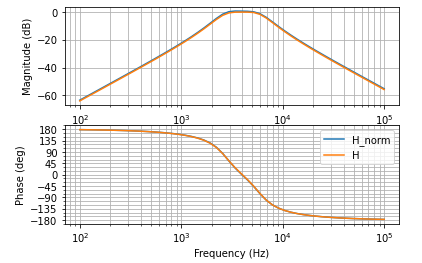
\includegraphics[width=\textwidth]{bode_norm.png}
\caption{Diagrama de bode (modulo y fase) normalizado}
\end{figure}

\begin{figure}[h]
\centering
	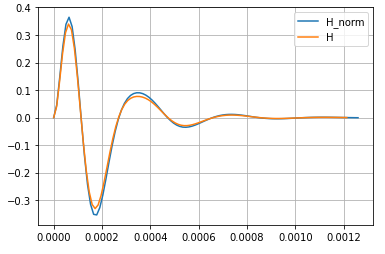
\includegraphics[width=\textwidth]{escalon_norm.png}
\caption{Respuesta al escalon normalizado}
\end{figure}

\newpage
\section*{Simulacion LTspice}
\begin{itemize}
\item Diagrama de Bode de modulo y fase
\begin{figure}[h]
\centering
	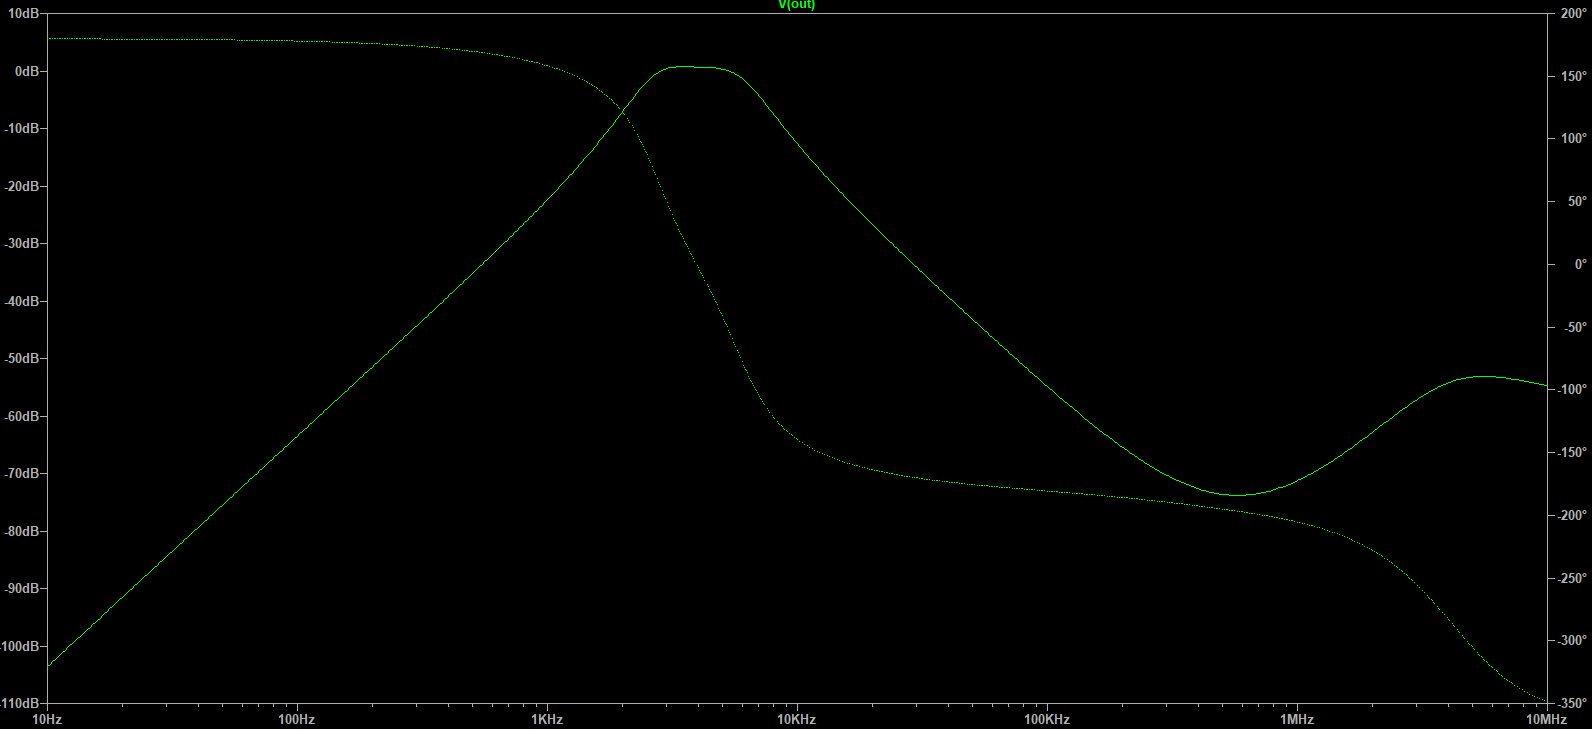
\includegraphics[width=\textwidth]{bode_TL081.png}
\caption{Diagrama de Bode ltspice}
\end{figure}

\newpage
\item Respuesta al escalon
\begin{figure}[h]
\centering
	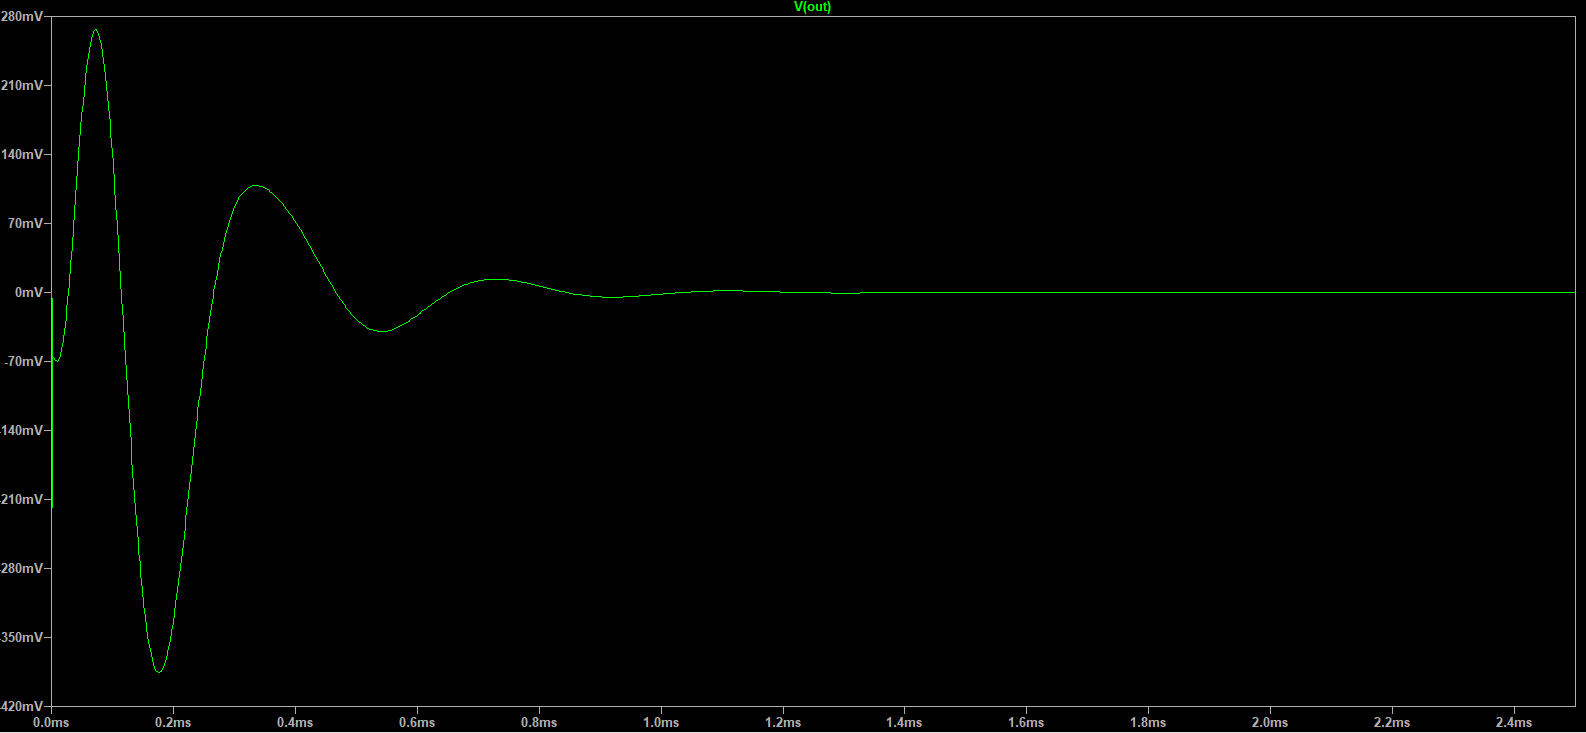
\includegraphics[width=\textwidth]{escalon_TL081.png}
\caption{Diagrama de Bode ltspice}
\end{figure}

\newpage
\item Respuesta a la senoidal
\begin{itemize}
\item f0
\begin{figure}[h]
\centering
	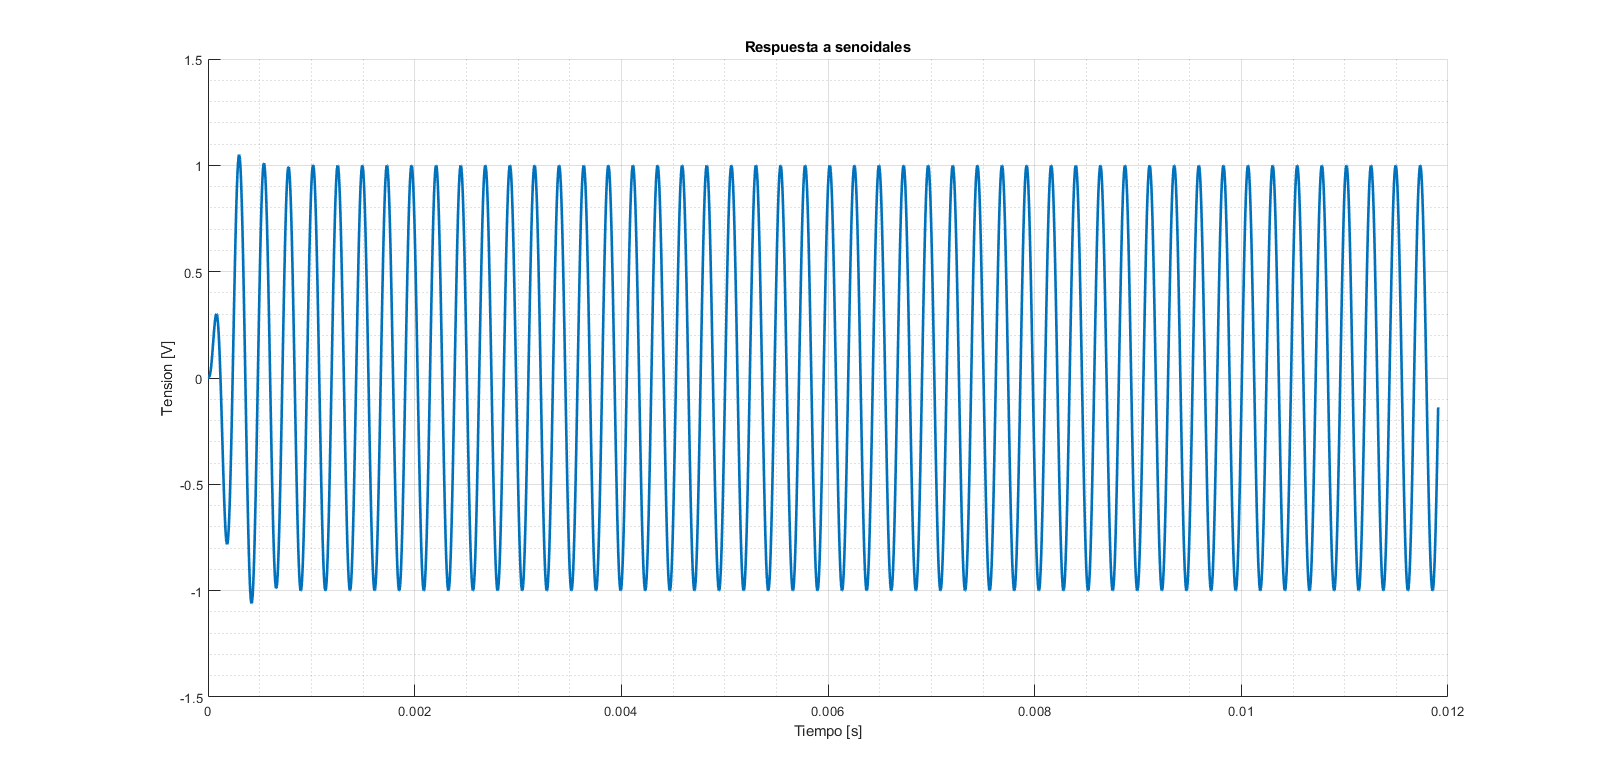
\includegraphics[width=\textwidth]{sen_fo_original.png}
\caption{Senoidal f0 original}
\end{figure}

\begin{figure}[h]
\centering
	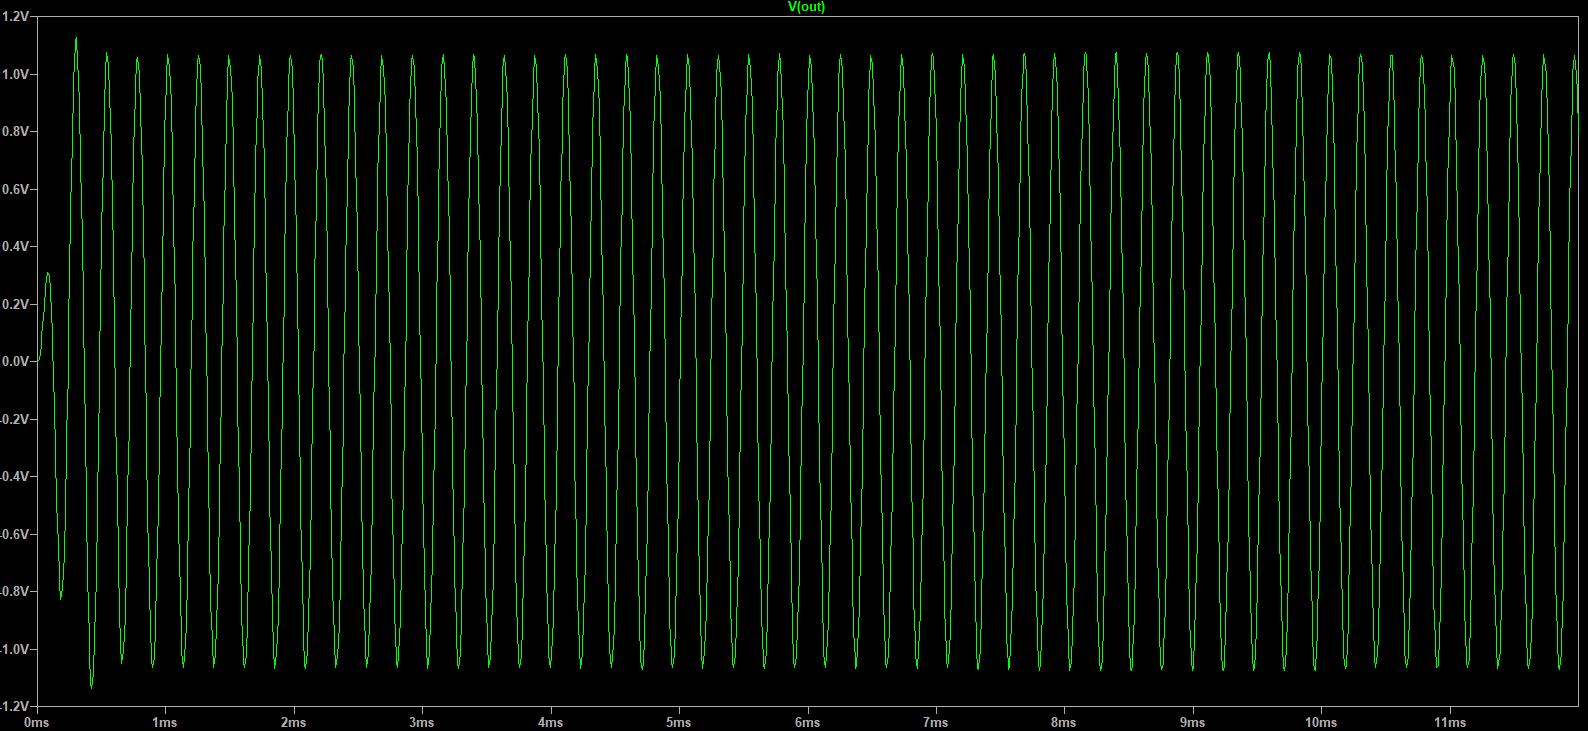
\includegraphics[width=\textwidth]{sen_fo_TL081.png}
\caption{Senoidal f0 TL081}
\end{figure}

\newpage
\item f0/10
\begin{figure}[h]
\centering
	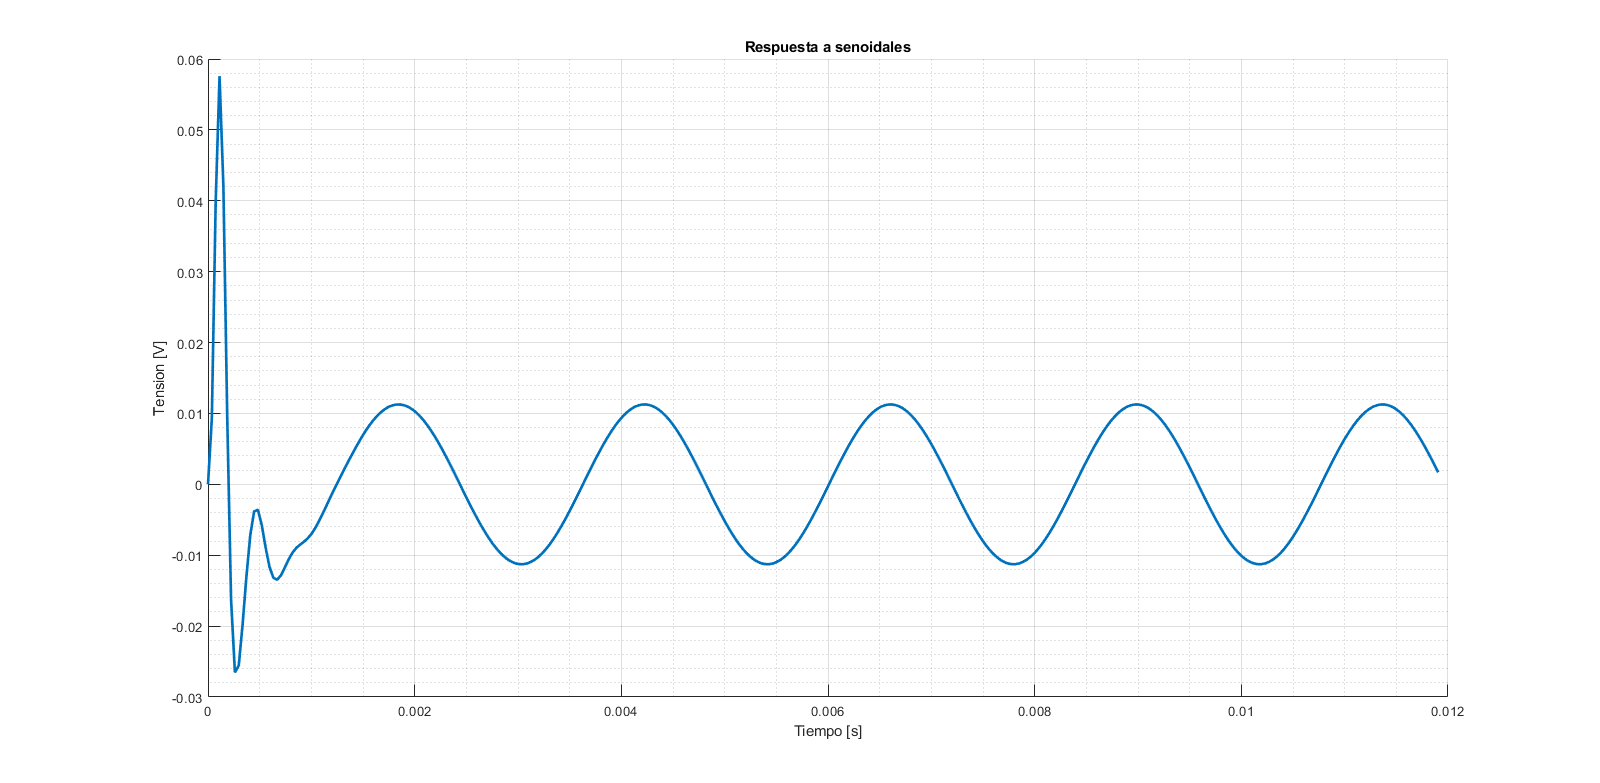
\includegraphics[width=\textwidth]{sen_fo_sobre_10_original.png}
\caption{Senoidal f0/10 original}
\end{figure}

\begin{figure}[h]
\centering
	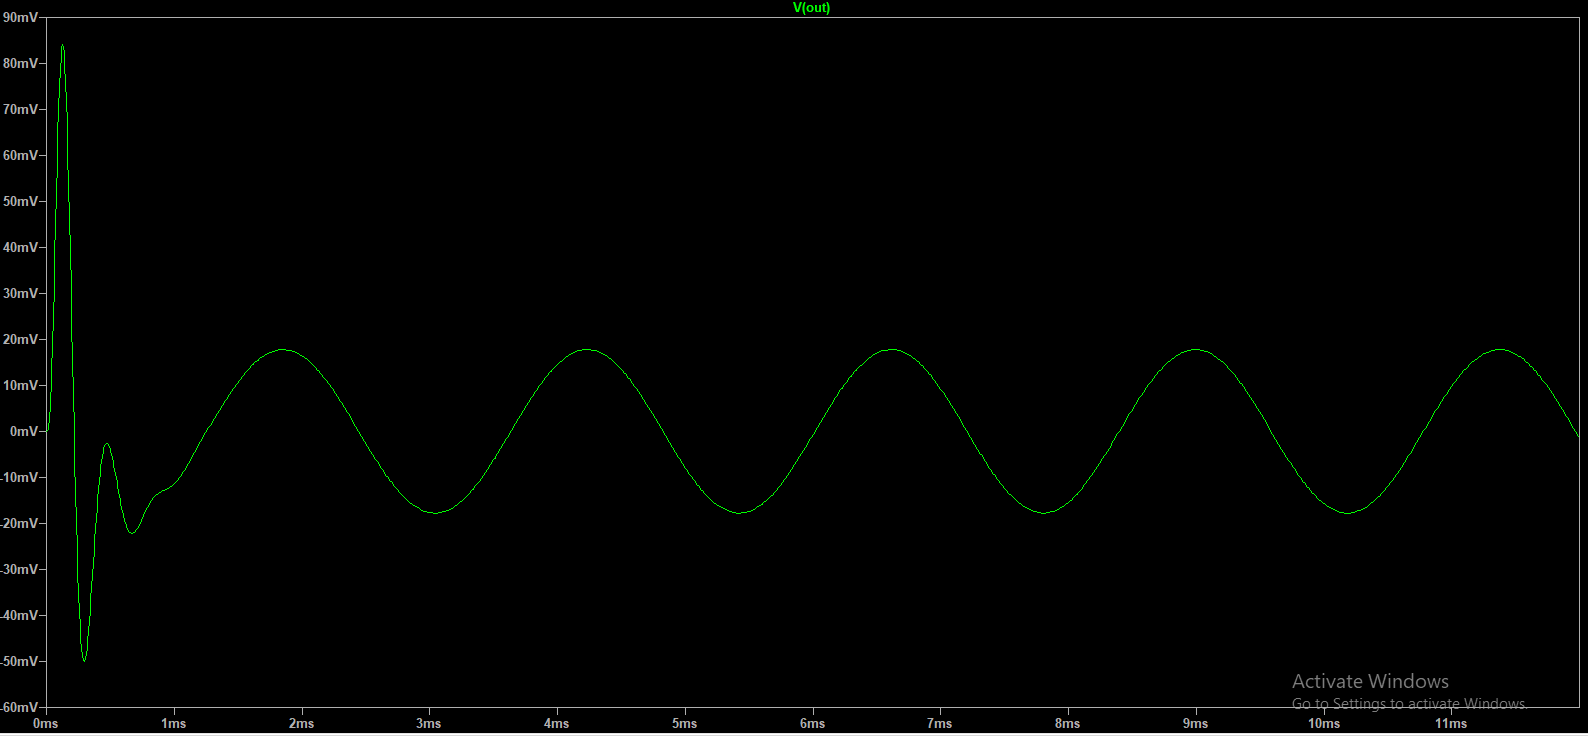
\includegraphics[width=\textwidth]{sen_fo_sobre_10_TL081.png}
\caption{Senoidal f0/10 TL081}
\end{figure}

\newpage
\item 10 $\cdot$ f0
\begin{figure}[h]
\centering
	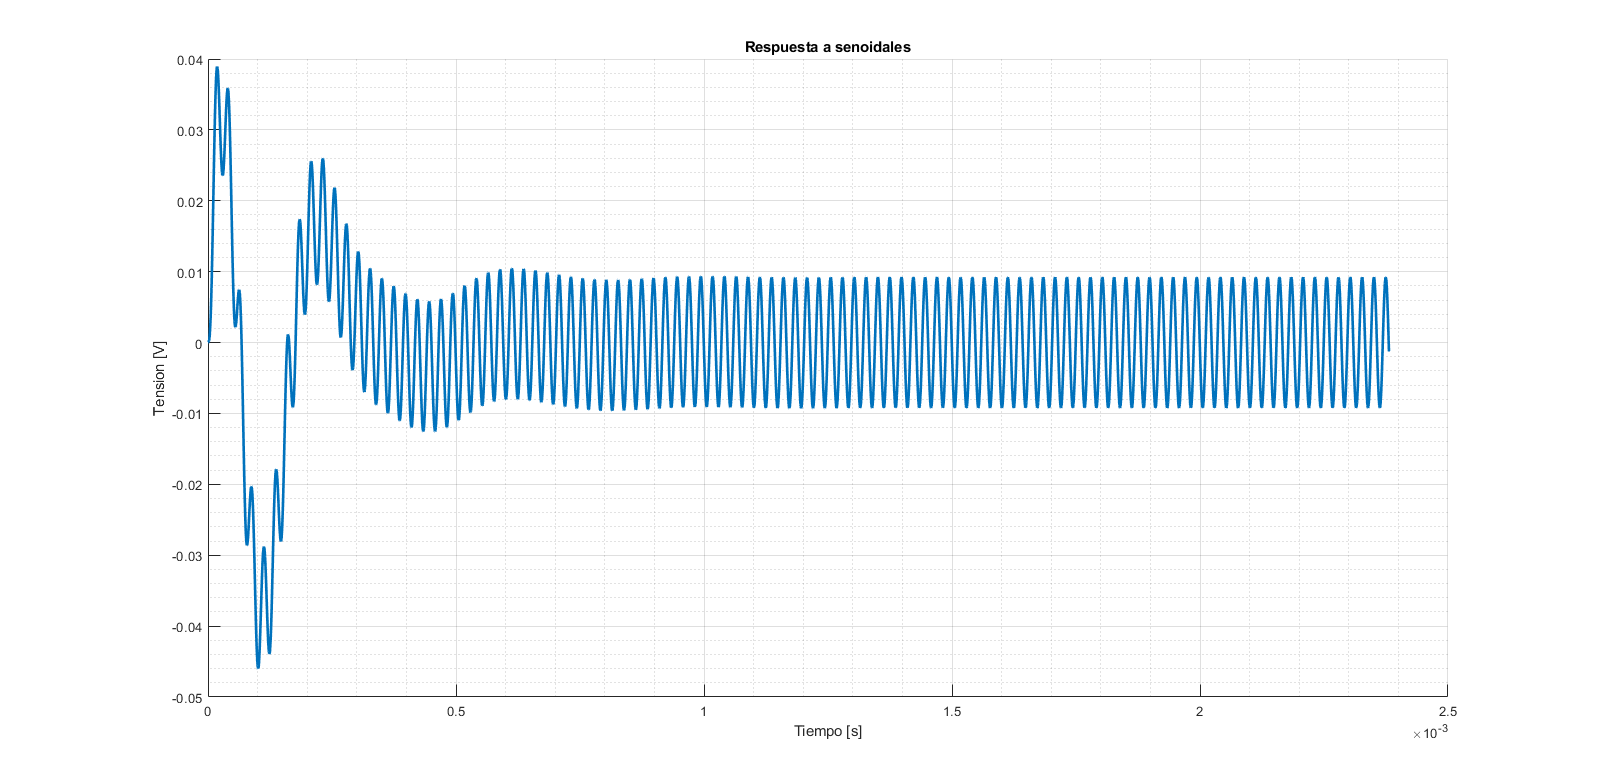
\includegraphics[width=\textwidth]{sen_fo_por_10_original.png}
\caption{Senoidal 10 $\cdot$ f0 original}
\end{figure}

\begin{figure}[h]
\centering
	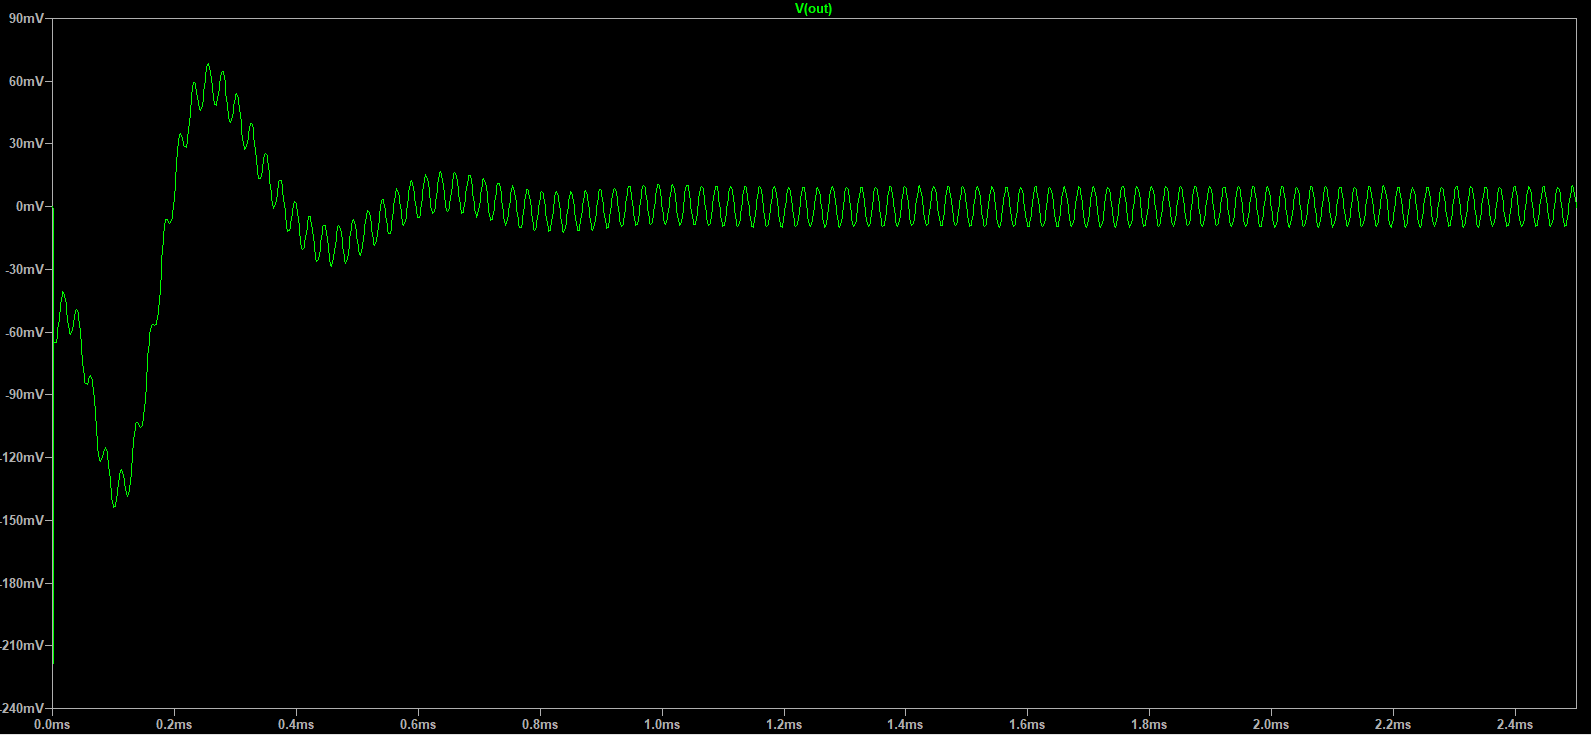
\includegraphics[width=\textwidth]{sen_fo_por_10_TL081.png}
\caption{Senoidal 10 $\cdot$ f0 TL081}
\end{figure}
\end{itemize}

\newpage
\item Respuesta a señal cuadrada
\begin{itemize}
\item f0
\begin{figure}[h]
\centering
	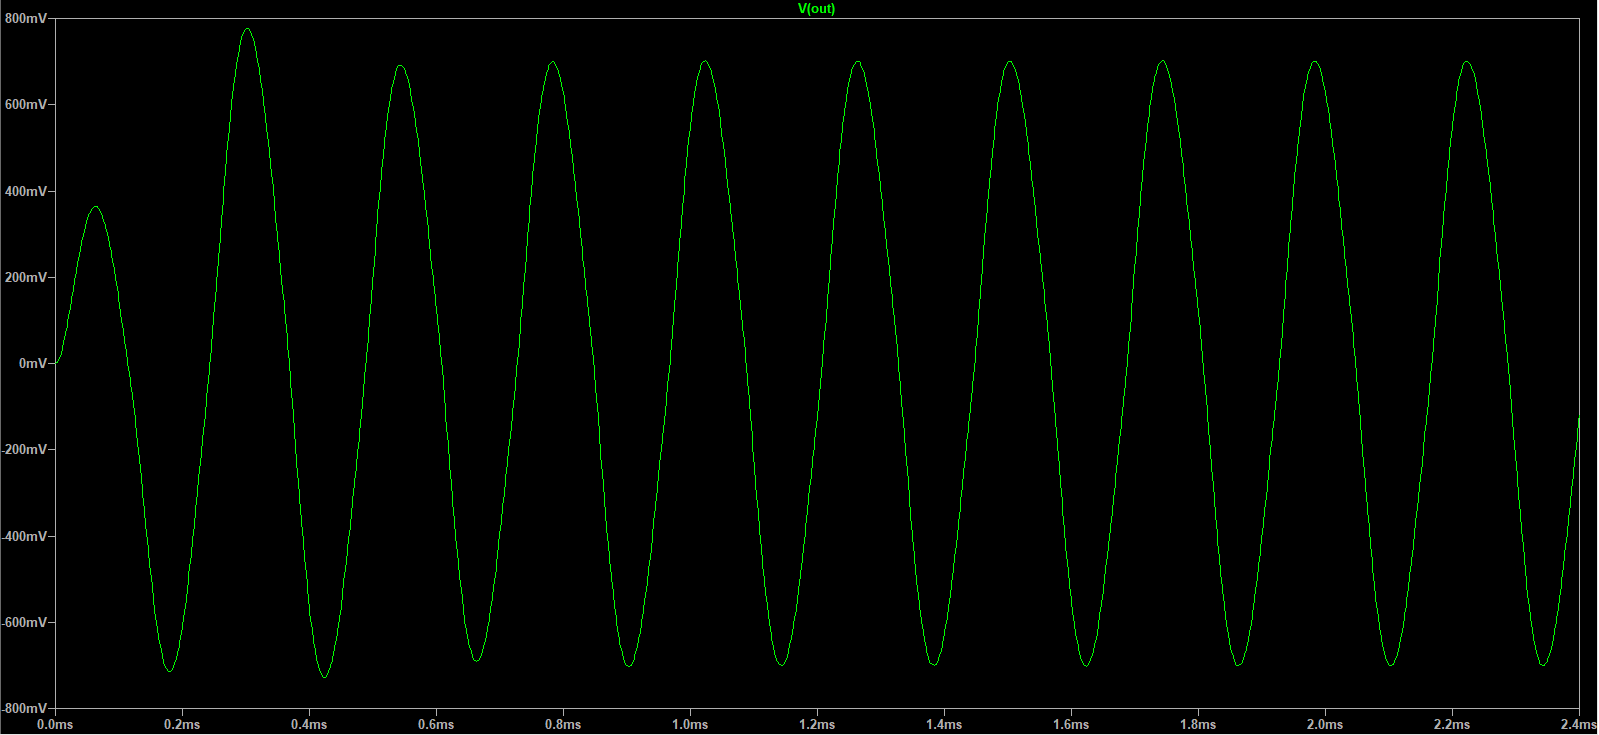
\includegraphics[width=\textwidth]{cuadrada_f0_TL081.png}
\caption{Cuadrada f0 TL081}
\end{figure}

\newpage
\item f0/10
\begin{figure}[h]
\centering
	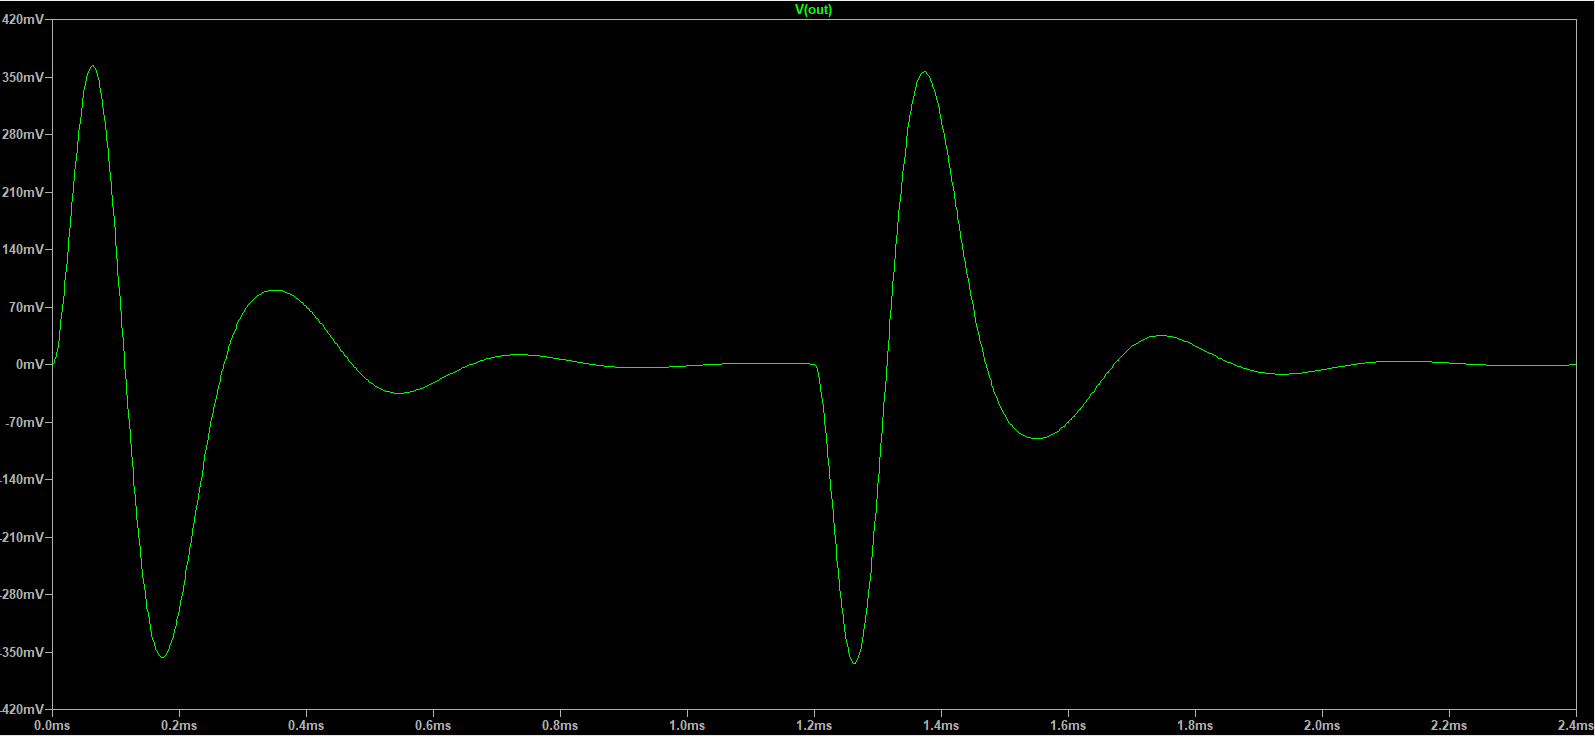
\includegraphics[width=\textwidth]{cuadrada_f0_sobre_10_TL081.png}
\caption{Cuadrada f0/10 TL081}
\end{figure}

\newpage
\item 10 $\cdot$ f0
\begin{figure}[h]
\centering
	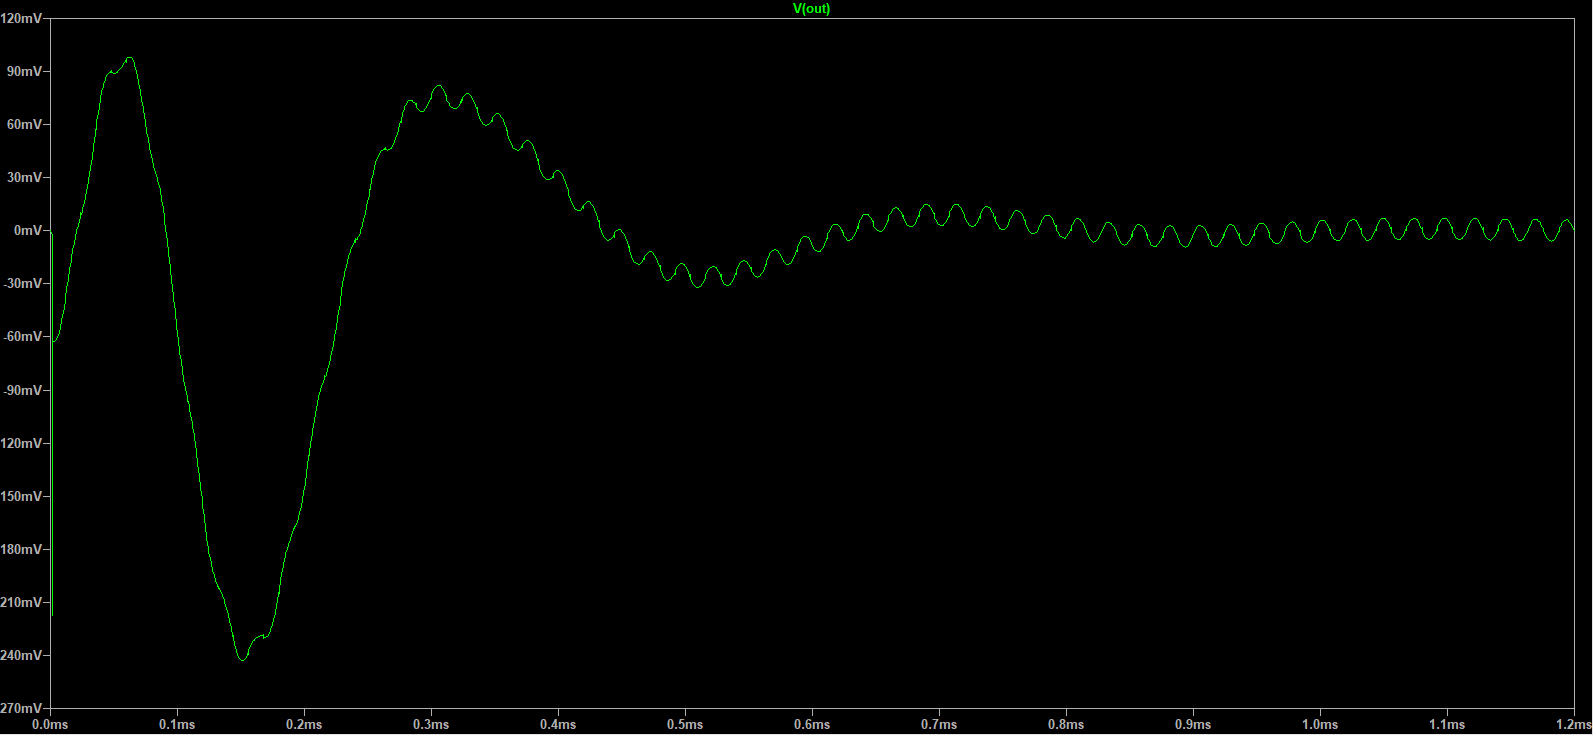
\includegraphics[width=\textwidth]{cuadrada_f0_por_10_TL081.png}
\caption{Cuadrada 10 $\cdot$ f0 TL081}
\end{figure}

\end{itemize}

\end{itemize}

%------------------------------------------------

\end{document}
